\chapter{Introduction}
\label{Ch:Introduction} %%%%%%%%%%%%%%%%%%%%%%%%%%%%
\graphicspath{{Figures/chapter1-Intro/}}

\thispagestyle{empty} % To avoid page numbering on Chapter 1

Speech is a natural form of communication among humans. Speech based \gls{hci}
is often preferred in personal digital assistants and home automation tools.
\Gls{asr} is the process of converting spoken utterances into textual form as a
sequence of words. \Gls{asr} systems have applications in generating captions
for videos, online meetings, transcribing lectures, speech based text input
systems, interactive voice response systems etc.

Speech recognition is a challenging problem that demands for addressing both the
acoustic and linguistic aspects of spoken language. This includes understanding
the physical properties of speech signals, as well as the linguistic structure
and meaning of the words and phrases being spoken. However the solutions to
linguistic challenges that are effective for one language cannot be easily
transferred to other languages. This is because natural human languages are so
diverse in terms of their typology, phonetic inventory, word vocabulary and in
digital resources. This thesis aims to address specific linguistic domain
challenges in the development of \gls{lvcsr} for Malayalam language. This
research work presents a comprehensive analysis of the challenges, in terms of
morphology and phonology, faced in building an \gls{asr} system for Malayalam
and proposes various tools and techniques to overcome them. Furthermore, these
proposed solutions have applications beyond ASR and can address some of the
generic problems in Malayalam \gls{nlp}.

\section{Background}

Digital devices and hardware are getting cheaper and easily available.
Utilisation of these devices to its full potential is possible only if every
user is able to communicate with these devices without barriers. A functional
\gls{asr} in one's native language is essential for speech based typing,
accessing speech enabled digital assistants and using interactive voice response
systems. This can be extended to applications like transcribing speech for the
hearing challenged and futuristic applications like speech to speech
translation.

The experiments used in this research work utilises the classical architecture of speech recognition described in Fig. \ref{fig:hybridASR}. Over the last three decades, the field of \gls{asr} has undergone significant advancements, with researchers focusing on optimising each component of the ASR architecture. Toolkits such as HTK \cite{young2002htk}, CMU Sphinx \cite{lee1990overview}, and Kaldi \cite{povey2011kaldi} have been developed based on this architecture, enabling researchers to integrate their work on improving individual components and evaluate their impact on the overall performance of the ASR system. 

\begin{figure}[h]
      \begin{center}
            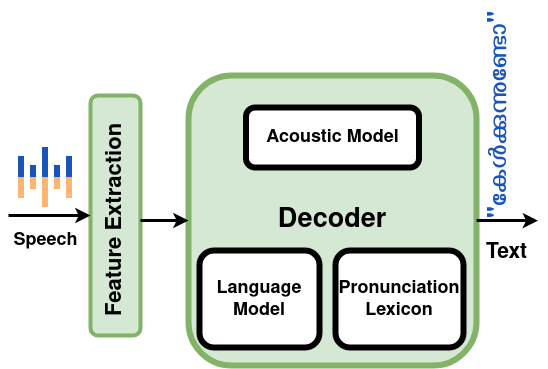
\includegraphics[width=0.7\textwidth]{ASR.png}
            \caption{Architecture of an ASR system}
            \label{fig:hybridASR}
      \end{center}
\end{figure}

In the context of this research on the morphologically complex Malayalam language, a significant challenge was encountered, stemming from the limited availability of annotated speech corpora under open licenses, thus positioning it as a low-resource language. Classical or pipeline architecture is best suited than the alternate \gls{e2e} architecture, in 
scenarios where text data outweighs audio data, a characteristic of the Malayalam language \cite{georgescu2021performance}. The research outcomes presented in \cite{bayerl2019comparison} and \cite{aku2021specom} indicate that attempting to train an \gls{e2e} \gls{asr} system from scratch, using a dataset comprising of less than 100 hours of annotated speech data, would lead to unsatisfactory accuracy. Additionally, the classical ASR models offer the advantage of easy integration into small hardware devices, enabling fast on-device speech recognition \cite{georgescu2021performance}. Thus, the research makes the deliberate choice to employ classical architecture over the \gls{e2e} approach, driven by the unique challenges and characteristics associated with the Malayalam language.

% Even though there are alternate architectures like \gls{e2e}, we stick to this pipeline model of speech recognition method for most of the experiments performed in this research. This was determined based
% on the data availability for building Malayalam \gls{asr}. Statistical or hybrid DNN/HMM methods are best suited for languages with limited labelled audio \cite{georgescu2021performance}. When much more text data is available than audio data, hybrid models are the preferred choice \cite{bayerl2019comparison,aku2021specom}.  



In the pipeline \gls{asr} system, the \gls{am} is the learnt
representation of relationship between the acoustic features of speech and the
phonemes of the language. The \gls{am} uses the \gls{gmm} to model the acoustic
features of speech and the \gls{hmm} to model the temporal structure of speech.
The GMM-HMM \gls{am} is trained on annotated speech data, and its parameters
are learned from the data using statistical techniques. The \gls{dnn} based
\gls{am} is an up-gradation over the conventional GMM-HMM approach of acoustic
modelling and is generally called DNN-HMM approach. The \gls{lm} is a model of
the probability distribution of words or subwords in the language. The \gls{lm}
is typically implemented as a statistical n-gram, which predicts the likelihood
of a sequence of words or subwords given the previous words in the sentence.
The \gls{pl} is a list of words or subwords in the language, along with the
corresponding phoneme level transcriptions. A detailed description of ASR
architectures is provided in Chapter \ref{Ch:Literature}.
% The \gls{pl} is used during the acoustic modelling step to map the speech signal to a sequence of units that are more closely aligned with the sounds of the target language.

\section{Motivation, Challenges and Proposed Solutions}

Malayalam is a Dravidian language spoken in the Indian state of Kerala and the union territories of Lakshadweep and Puducherry. It is one of the twenty two scheduled languages of India spoken by nearly 2.88\% of Indians, with more than thirty five million speakers across the globe. Malayalam has the official language status in the state of Kerala and in the union
territories of Lakshadweep and Puducherry (Mahé). Malayalam has been designated as a classical language in India since
2013\footnote{\url{https://en.wikipedia.org/wiki/Malayalam}} due to its rich literary heritage and cultural significance. 

However, despite a huge number of speakers, based on our investigations and survey of reported literature, it is understood that Malayalam is a low-resourced language for the  following reasons \cite{besacier2014automatic}:

\begin{enumerate}
    \item Limited  availability of  linguistic resources, like
    \begin{enumerate}
        \item Lexical resources. eg: Machine-readable dictionaries.
        \item Linguistic corpora. eg: Transcribed speech corpus \cite{bhogale2023effectiveness} and parallel text corpus.
        \item Linguistically annotated corpora. eg: part-of-speech tagged text corpus.
    \end{enumerate}
    \item Lack of tools for creating linguistic resources manually or semi-automatically \footnote{\url{https://en.wikipedia.org/wiki/Language_resource}}.
    \item Lack of benchmark datasets for comparison of results.
\end{enumerate}




The field of speech recognition for the Malayalam language has not yet reached maturity and is not ready for real-world applications due to a variety of reasons, including
a shortage of annotated speech data and a lack of computational linguistic resources that can address the unique morphological and phonological features of the Malayalam language.

% \section{Specific Challenges and Proposed Solutions}

The morphological complexity in the word formation rules in Malayalam practically makes its vocabulary unlimited \cite{bharadwaja2007statistical}. Each root word can give rise to hundreds of derived words by agglutination, inflection and compounding \cite{thottingal2019finite}. Additionally, loan words  from other languages and proper nouns get added to the
vocabulary very fast in modern days. 
% There has not been any reported work on Malayalam \gls{lvcsr}, that can handle a vocabulary of more than 27500 words (Details presented in Section \ref{sec:Literature-malayalamasr}).
The grapheme to phoneme correspondence in Malayalam is not truly
one-to-one (See Appendix \ref{app:app1} for details). A static \gls{pl} used to build an ASR decoder may not be sufficient to handle words the system may encounter in the future. It will also be required to update the \gls{pl}, with new words from time to time. All of this leads to the necessity for an automated \gls{g2p} conversion tool and this research work proposes and implements its development.


% A \gls{pl} is an essential component in the building of a pipeline \gls{asr} system. 
%  A detailed description of this is made in Appendix \ref{app:app1}.
% It is not practical to create a hand curated large vocabulary
% pronunciation lexicon. Additionally 

The challenges of the morphological complexity of the language
can be addressed by open vocabulary speech recognition. This refers to the use
of subword based language models and lexicons instead of word based ones \cite{creutz2007analysis}. This
method effectively handles each word by  decomposing it to
subwords and then reconstructing them back to words after decoding. This research work proposes and implements linguistically informed subword modelling algorithms and compare their effectiveness in Malayalam \gls{asr} task.

% The lack of huge annotated Malayalam speech corpora makes it a resource scarce language prohibiting the exploration of modern \gls{e2e} \gls{asr} models for Malayalam.

% To design and develop a hybrid \gls{lvcsr} system, diverse language resources are needed. A parallel corpus of recorded speech and its textual transcription, text data corpus, phonetic lexicon are the three essential language resources needed for developing an \gls{asr} system.  The building process of \gls{asr} systems requires transcribed speech recordings from many speakers, pronunciation dictionaries which cover the full vocabulary of at least the training corpus, and massive amounts of text data to reliably train statistical language models \cite{besacier2014automatic}.

% An algorithmic modelling of the pronunciation rules of Malayalam language is essential to build a bidirectional grapheme - phoneme conversion tool in Malayalam. The algorithm development process is to be guided by a linguistic research on the phonetic properties of Malayalam script. A quantitative analysis of the morphological complexity is essential in analysing the reasons behind comparatively high error rates in Malayalam \gls{asr}  and in the quest for solving them using an open vocabulary speech recognition system. 

\section{Research Objective}

The focus of this research is on the the investigation of the linguistic
challenges associated with \gls{asr} in Malayalam language and the development
of open source computational linguistic tools and techniques essential to solve
them. Specifically the objectives can be described as:

\begin{enumerate}
      \item To analyse the morphological complexity of Malayalam and the challenges it
            imposes on building a continuous speech recognition system.
      \item To automate the process of creating a large vocabulary pronunciation lexicon
            taking care of precise grapheme to phoneme conversion rules of Malayalam.
      \item To build a \gls{lvcsr} model for Malayalam using the pipeline architecture,
            combining a large vocabulary pronunciation lexicon, a hybrid DNN-HMM acoustic
            model and a statistical language model.
      \item To build an open vocabulary \gls{asr} system for Malayalam using subword based
            \gls{pl} and \gls{lm} to reduce the impact of morphological complexity.

\end{enumerate}

\section{Contributions of this Thesis}

Considering the challenges involved in an \gls{asr} system
for Malayalam, this research has contributed towards the development of an open
and functional \gls{asr} model for Malayalam that could be integrated to
various tasks. The major contributions are:
\begin{enumerate}
      \item Quantitative analysis of the morphological complexity of Malayalam language.
      \item Documentation of the graphemic and phonemic inventory of Malayalam and the
            correspondence between the two.
      \item  Development of an algorithmic description of the grapheme-phoneme
            correspondence in Malayalam and its implementation into a modular toolkit which may find applications in script grammar check, orthographic syllabification, phonetic feature analysis, grapheme to phoneme and phoneme to grapheme conversions.
      \item  Publication of large vocabulary pronunciation lexicon of more than hundred thousand words belonging to different word categories.
      \item Development of a \gls{lvcsr} model for Malayalam and publication of an open licensed Malayalam \gls{asr} model that could be integrated to various
            applications.
      \item Exploration of subword segmentation strategies suited for Malayalam considering its morphological complexity.
      \item  Development of subword based open vocabulary \gls{asr} model to reduce
            \gls{wer} and model memory requirement.
\end{enumerate}



Furthermore, open dissemination of the source codes and the developed models is very much essential to ensure reproducibility, reusability, and most importantly for validation and further improvements, leading to research continuity. This aspect 
has been given utmost priority at every stage of this research work.

% \section{Major Contributions}

% A speech recognition system in general has a structure shown in Figure \ref{ASR}. The  \textbf{Acoustic Models} and \textbf{Language Models} are pretrained on a large speech and text corpora. \textbf{Pronunciation Lexical model} assigns each orthographic token with one or more phonetic transcription.
% During speech decoding, the input speech is represented as a sequence of acoustic features and matched with the pretrained models, to generate a sequence of words. There are several open source toolkits that enable model training and decoding process. HTK\footnote{\url{http://htk.eng.cam.ac.uk/}}, CMUSphinx\footnote{\url{https://sourceforge.net/projects/cmusphinx/}}, Kaldi\footnote{\url{https://kaldi-asr.org/doc/}} etc. are to name a few.

\section{Organisation of the Thesis}

The chapter \ref{Ch:Introduction} of this thesis highlights the motivation,
specific challenges, research objectives and the contributions of this work.
Chapter \ref{Ch:Literature} reviews the related works on general \gls{asr}
system architectures, \gls{g2p} conversion systems, morphology aware \gls{asr}
systems, Malayalam speech corpora and Malayalam \gls{asr} systems.

Chapter \ref{Ch:MorphologicalComplexity} describes the quantitative analysis on
the morphological complexity of Malayalam language. This analysis suggested two potential directions for research. The first involves developing a tool to create large vocabulary pronunciation lexicons, while the second involves implementing subword based ASR techniques. 

Chapter \ref{ch:Mlphon} explains the design and development of bidirectional \gls{g2p} toolkit Mlphon. The chapter also presents the evaluation of the toolkit intrinsically on a gold standard lexicon and the \gls{nlp} applications of this toolkit. Chapter \ref{ch:lvcsr} presents the development of an \gls{lvcsr} system for
Malayalam with a large vocabulary pronunciation lexicon created using Mlphon,
acoustic and language models trained using various openly licensed speech and
text datasets. It also presents a comparison of the \gls{asr} results with
other lexicon creation tools.

% Chapter \ref{ch:NatureofOrthography} gives an overview of the nature of Malayalam orthography, the phonetic inventory of the language and the correspondence between the graphemes and phonemes of the language.



Chapter \ref{ch:openvocab} explores different
subword segmentation strategies for \gls{asr} in Malayalam
language. Chapter \ref{ch:conclusion} concludes the thesis highlighting the
contributions, limitations and listing the scope for future research work.

A detailed documentation of the graphemic and phonemic inventory of Malayalam is provided in Appendix \ref{app:app1}.
% and the algorithmic description of the relationship between the two in a form that could be implemented using finite state transducers is given in Appendix \ref{app:app2}. 
It is followed by the list of references and the list of publications based on the findings in this thesis. 